\chapter{Introduction}

This book will start you on the long and difficult trek to becoming a modern
problem solver. Along the path, you will learn how to use the tools of
math, computers, and science. 

Why should you bother? There are big problems in this world that will
require expert problem solvers. Those people will make the world a
better place while enjoying interesting and lucrative careers. We are
talking about engineers, scientists, doctors, computer programmers,
architects, actuaries, and mathematicians. Right now, those occupations represent
about 6\% of all the jobs in the United States. Soon,
that number is expected to rise above 10\%.  On average, people in
that 10\% of the population are expected to have salaries twice that
of their non-technical counterparts.\index{career}

Solving problems is difficult. At some point on this journey, you will
see people who are better at solving problems than you are. You, like
every other person who has gone on this journey, will think ``I have
worked so hard on this, but that person is better at it than
I am. I should quit.'' Don't.\index{quitting}

First, solving problems is like a muscle. The more you do, the better
you get at it.  It is OK to say ``I am not good at this yet.'' That
just means you need more practice.

Second, you don't need to be the best in the world. 10 million people
your age can be better at solving problems than you, \textit{and you
  can still be in the top 10\% of the world}. If you complete this
journey, there will be problems for you to solve and a job where your
problem-solving skills will be appreciated.

So where do we start?

\section{Atoms}

The famous physicist Richard Feynman once asked this question: ``If,
in some cataclysm, all of scientific knowledge were to be destroyed,
and only one sentence was passed on to the next generation of
creatures, what statement would contain the most information in the
fewest words?''

His answer was ``All things are made of atoms—little particles that move around in
perpetual motion, attracting each other when they are a little
distance apart, but repelling upon being squeezed into one another.''

That seems like a good place to start.\index{atom}

All things (including the air around you) are made of atoms. Atoms are
very tiny -- there are more atoms in a drop of water than there are
drops of water in all the oceans.
% ADD: If you want a better visual of the scale: https://htwins.net/scale2/, start at around 10^-8

Every atom has a nucleus that contains protons and neutrons. There is also
a cloud of electrons flying around the nucleus. However, the mass of the atom
comes mainly from the protons and neutrons, which are exponentially heavier
than electrons.\index{protons} \index{neutrons} \index{electrons}

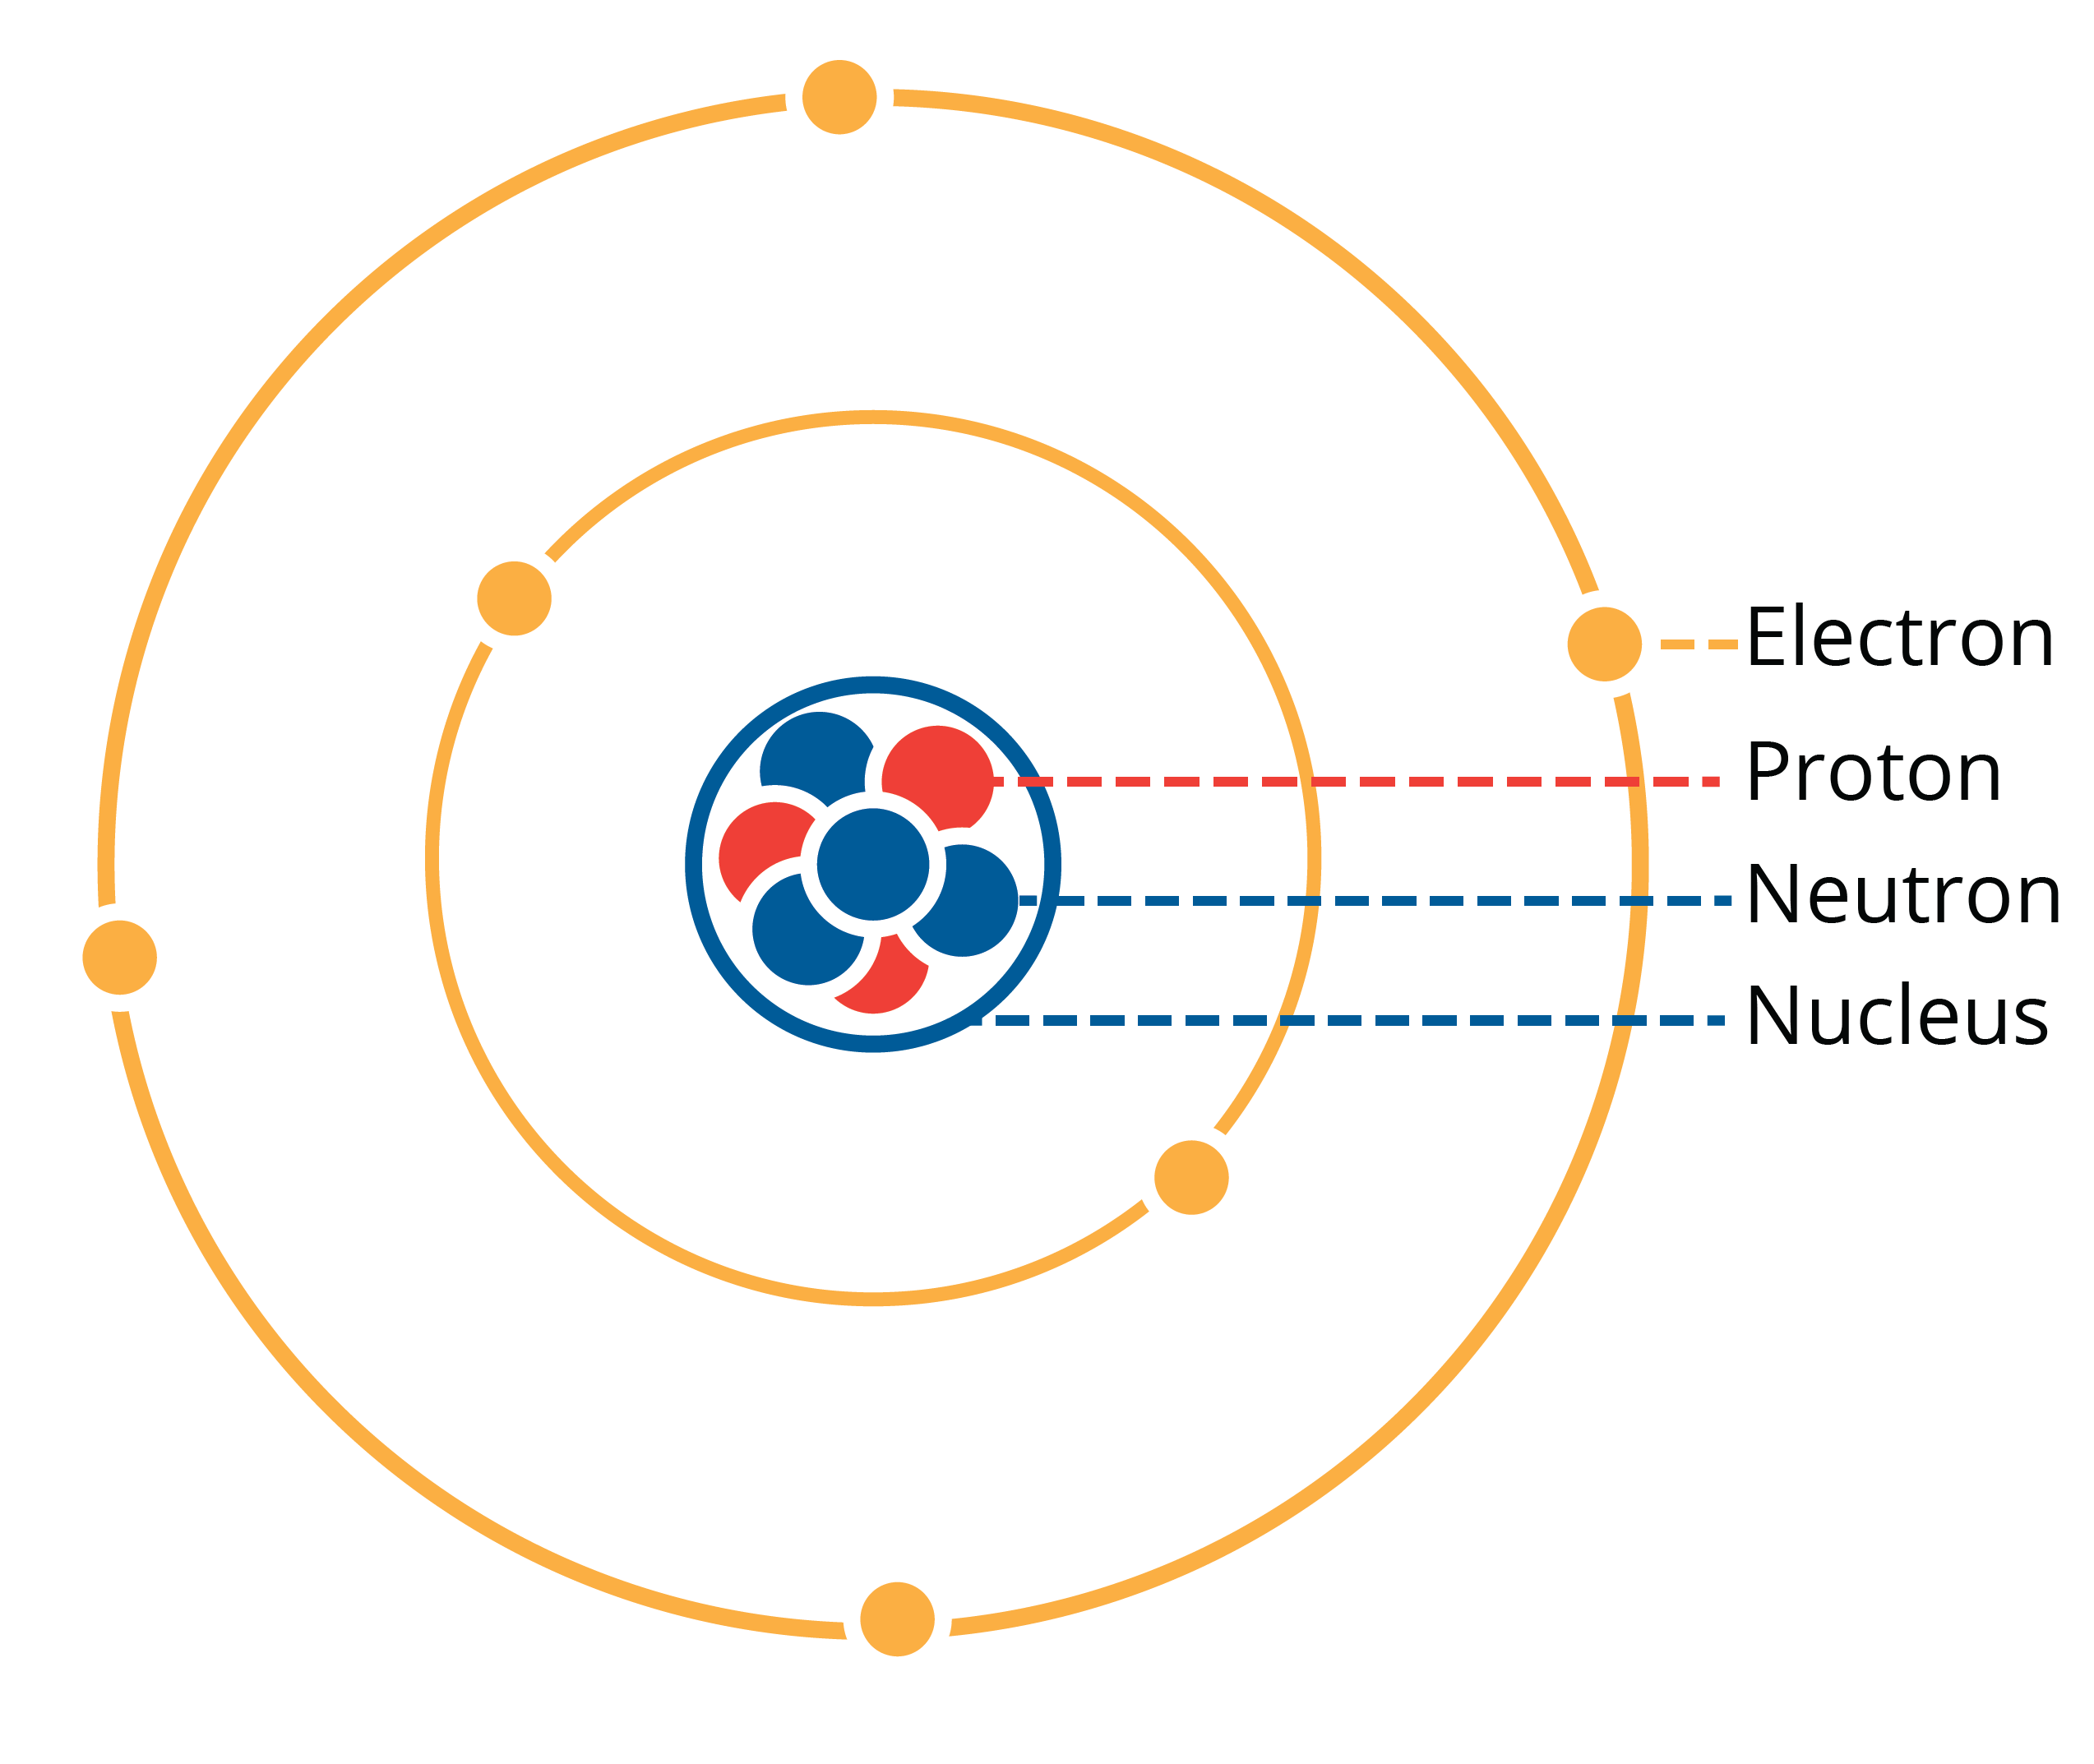
\includegraphics[width=.5\textwidth]{atom1.png}

Watch \textbf{Elements and atoms} from Khan Academy at \url{https://youtu.be/IFKnq9QM6_A}.

% ADD: Maybe get into different representaions of the atom: plum pudding, nuclear, planetary, quantum 

We classify atoms by the numbers of protons they have. An atom with one proton is a
hydrogen atom, an atom with two protons is a helium atom, and so forth (refer to periodic table on pg..). We say that hydrogen and helium are

\textit{elements} because the classification of elements is based on proton number. And we give
each element an atomic symbol. Hydrogen gets $H$. Helium gets $He$ Oxygen gets
$O$. Carbon gets $C$\index{elements}, etc.

Often two hydrogen atoms will attach to an oxygen atom. The result is
a water molecule. Why do they cluster together? because they share 
electrons in their clouds.\index{molecules}
% ADD:Electronegativity

A molecule is described by the elements it contains. Water is $H_2O$
because it has two hydrogen atoms and one oxygen atom.

There are many kinds of molecules. You know a few:
\begin{itemize}
\item Table salt is crystals made of $NaCl$ molecules: a sodium atom attached to a chlorine atom.
\item Baking soda, or sodium bicarbonate, is $NaHCO_3$.
\item Vinegar is a solution including acetic acid ($CH_3COOH$).
\item $O_2$ is the oxygen molecules that you breathe out of the air (Air, a blend of gases, is mostly $N_2$.).
\end{itemize}


Sometimes two hydrogen atoms form a molecule ($H_2$). Sometimes two
oxygen atoms form a molecule ($O_2$). If you mix these
together and light a match, they will rearrange themselves into water
molecules. This is called a \textit{chemical reaction}.  In any
chemical reaction, the atoms are rearranged into new molecules.\index{chemical reaction}
% ADD: electronegativity

Some chemical reactions (like the burning of hydrogen gas described
above) are \textit{exothermic} -- that is, they give off energy.
Burning hydrogen gas happens quickly and gives off a lot of energy. If
you have enough, it will make quite an explosion.\index{exothermic}
% ADD: endo/ exo thermic graphs/ explination

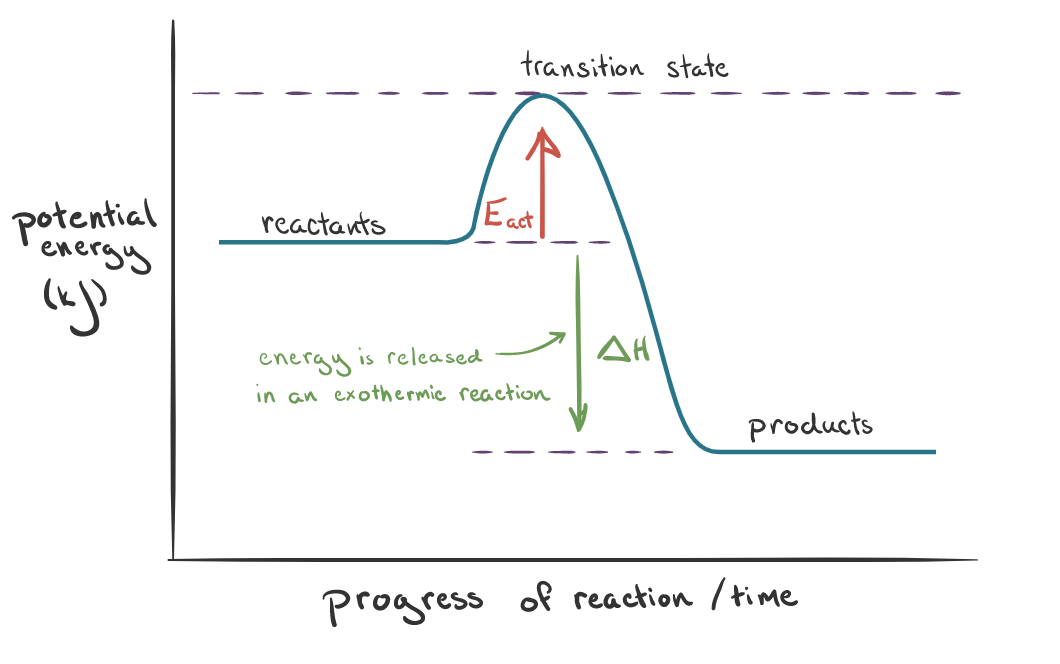
\includegraphics[width=0.7\textwidth]{KA_Exo.png}

Other chemical reactions are \textit{endothermic} -- that is they consume
energy.  Photosynthesis, the process by which plants consume energy
from the sun to make sugar from $CO_2$ and $H_2O$ requires an endothermic
chemical reaction.\index{endothermic}

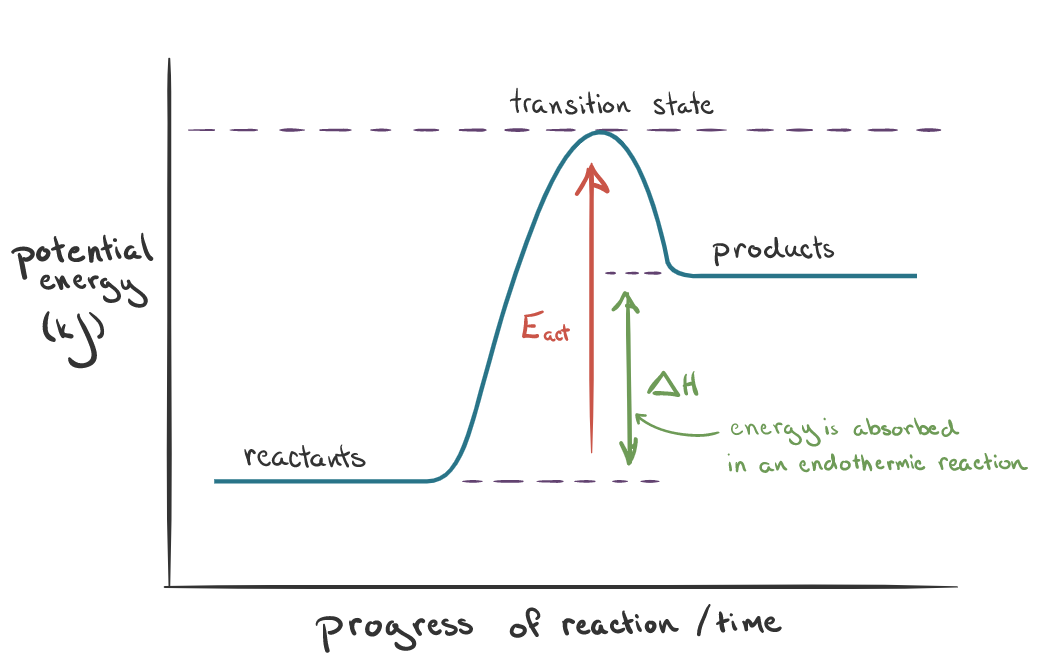
\includegraphics[width=0.7\textwidth]{KA_Endo.png}

\section{Mass and Acceleration}

Each atom has a mass, so everything that is made up of atoms has a
mass, which is pretty much everything.  We measure mass in grams.  A
paper clip is about 1 gram of steel. An adult human can weigh 70,000
grams, so for larger things we often talk about kilograms. A kilogram
is 1000 grams.

The first interesting thing about mass is that objects with more mass
require more force to accelerate. For example, pushing a bicycle so
that it accelerates from a standstill to jogging speed in 2 seconds
requires a lot less force than pushing a train so that it accelerates
at the same rate.

You will probably find it useful to watch Khan Academy's summary of
Newton's second law of motion: \url{https://youtu.be/ou9YMWlJgkE}

\begin{mdframed}[style=important, frametitle={Newton's Second Law of Motion}]

The force necessary to accelerate an object of mass $m$ is given by:

$$F = m a$$

That is the force is equal to the mass times the acceleration.

\end{mdframed}

What are the units here? We already know that mass is measured in
kilograms. We can measure velocity in meters per second, but that is
different from acceleration. Acceleration is the rate of change in
velocity. So if we want to go from 0 to 5 meters per second (that's
jogging speed) in two seconds. That is a change in velocity of 2.5
meters per second every second. We would say this acceleration is $2.5
m/s^2$.

What about measuring force? Newton decided to name the unit after
himself: The force necessary to accelerate one kilogram at $1 m/s^2$
is known as \textit{a newton}.

\begin{Exercise}[title={Acceleration}, label=acceleration_train]
  
While driving a bulldozer, you come across a train car (with no brakes
and no locomotive) on a track in the middle of a city. The train car
has a label telling you that it weighs 2,400 kg. There is a bomb
welded to the interior of the train car, and the timer tells you that
you can safely push the train car for 120 seconds. To get the train
car to where it can explode safely, you need to accelerate it to 20 meters per
second. Fortunately, the track is level and the train car's wheels have
almost no rolling resistance.

With what force, in newtons, do you need to push the train for those 120 seconds?

\end{Exercise}
\begin{Answer}[ref=acceleration_train]
To get the train to 20 meters per second in 120 seconds, you must
accelerate it with a constant rate of $\frac{1}{6} m/s^2$. You
remember that $F = m a$, so $F = 2400 \times \frac{1}{6}$. Thus, you
will push the train with a force of 400 newtons for the 120 seconds
before the bomb goes off.
\end{Answer}

\section{Mass and Gravity}

The second interesting thing about mass is that masses are
attracted to each other by the force we call \textit{gravity}. The
force of attraction between two objects is proportional to the product
of their masses. As objects get farther away, the force decreases.
That is why you are more attracted to the earth than you are to
distant stars, which have much more mass than the earth.
%ADD: Collums Law

\begin{mdframed}[style=important, frametitle={Newton's Law of Universal Gravitation}]

Two masses ($m_1$ and $m_2$) that are a distance of
$r$ from each other, are attracted toward each other with a force of
magnitude:

$$F = G\frac{m_1 m_2}{r^2}$$

where $G$ is the universal gravitational constant. If you measure the
mass in kilograms and the distance in meters. $G$ is about $6.674
\times 10^{-11}$.  That will get you the force of the attraction in
newtons.

\end{mdframed}

\begin{Exercise}[title={Gravity}, label=gravity_earth]
  
  The earth's mass is about $6 \times 10^{24}$ kilograms.

  Your spacecraft's mass is 6,800 kilograms.

  Your spacecraft is also about 100,000 km from the center of the earth. (For reference, the moon is about 400,000 km from the center of the earth.)

  What is the force of gravity that is pulling your spacecraft and the earth toward each other?

\end{Exercise}
\begin{Answer}[ref=gravity_earth]

  $$F = G\frac{m_1 m_2}{r^2} = (6.674 \times 10^{-11})\frac{(6.8 \time 10^3)(6 \times 10^{24})}{(10^5)^2} = 6.1 \times 10^{6}$$

  About 6 million newtons.
  
\end{Answer}

\section{Mass and Weight}

Gravity pulls on things proportional to their mass, so we often
ignore the difference between mass and weight.

The weight of an object is the force due to the object's mass and
gravity.  When we say, ``This potato weighs 1 pound,'' we actually mean
``This potato weighs 1 pound on earth.''  That same potato would weigh
about one-fifth of a pound on the moon.

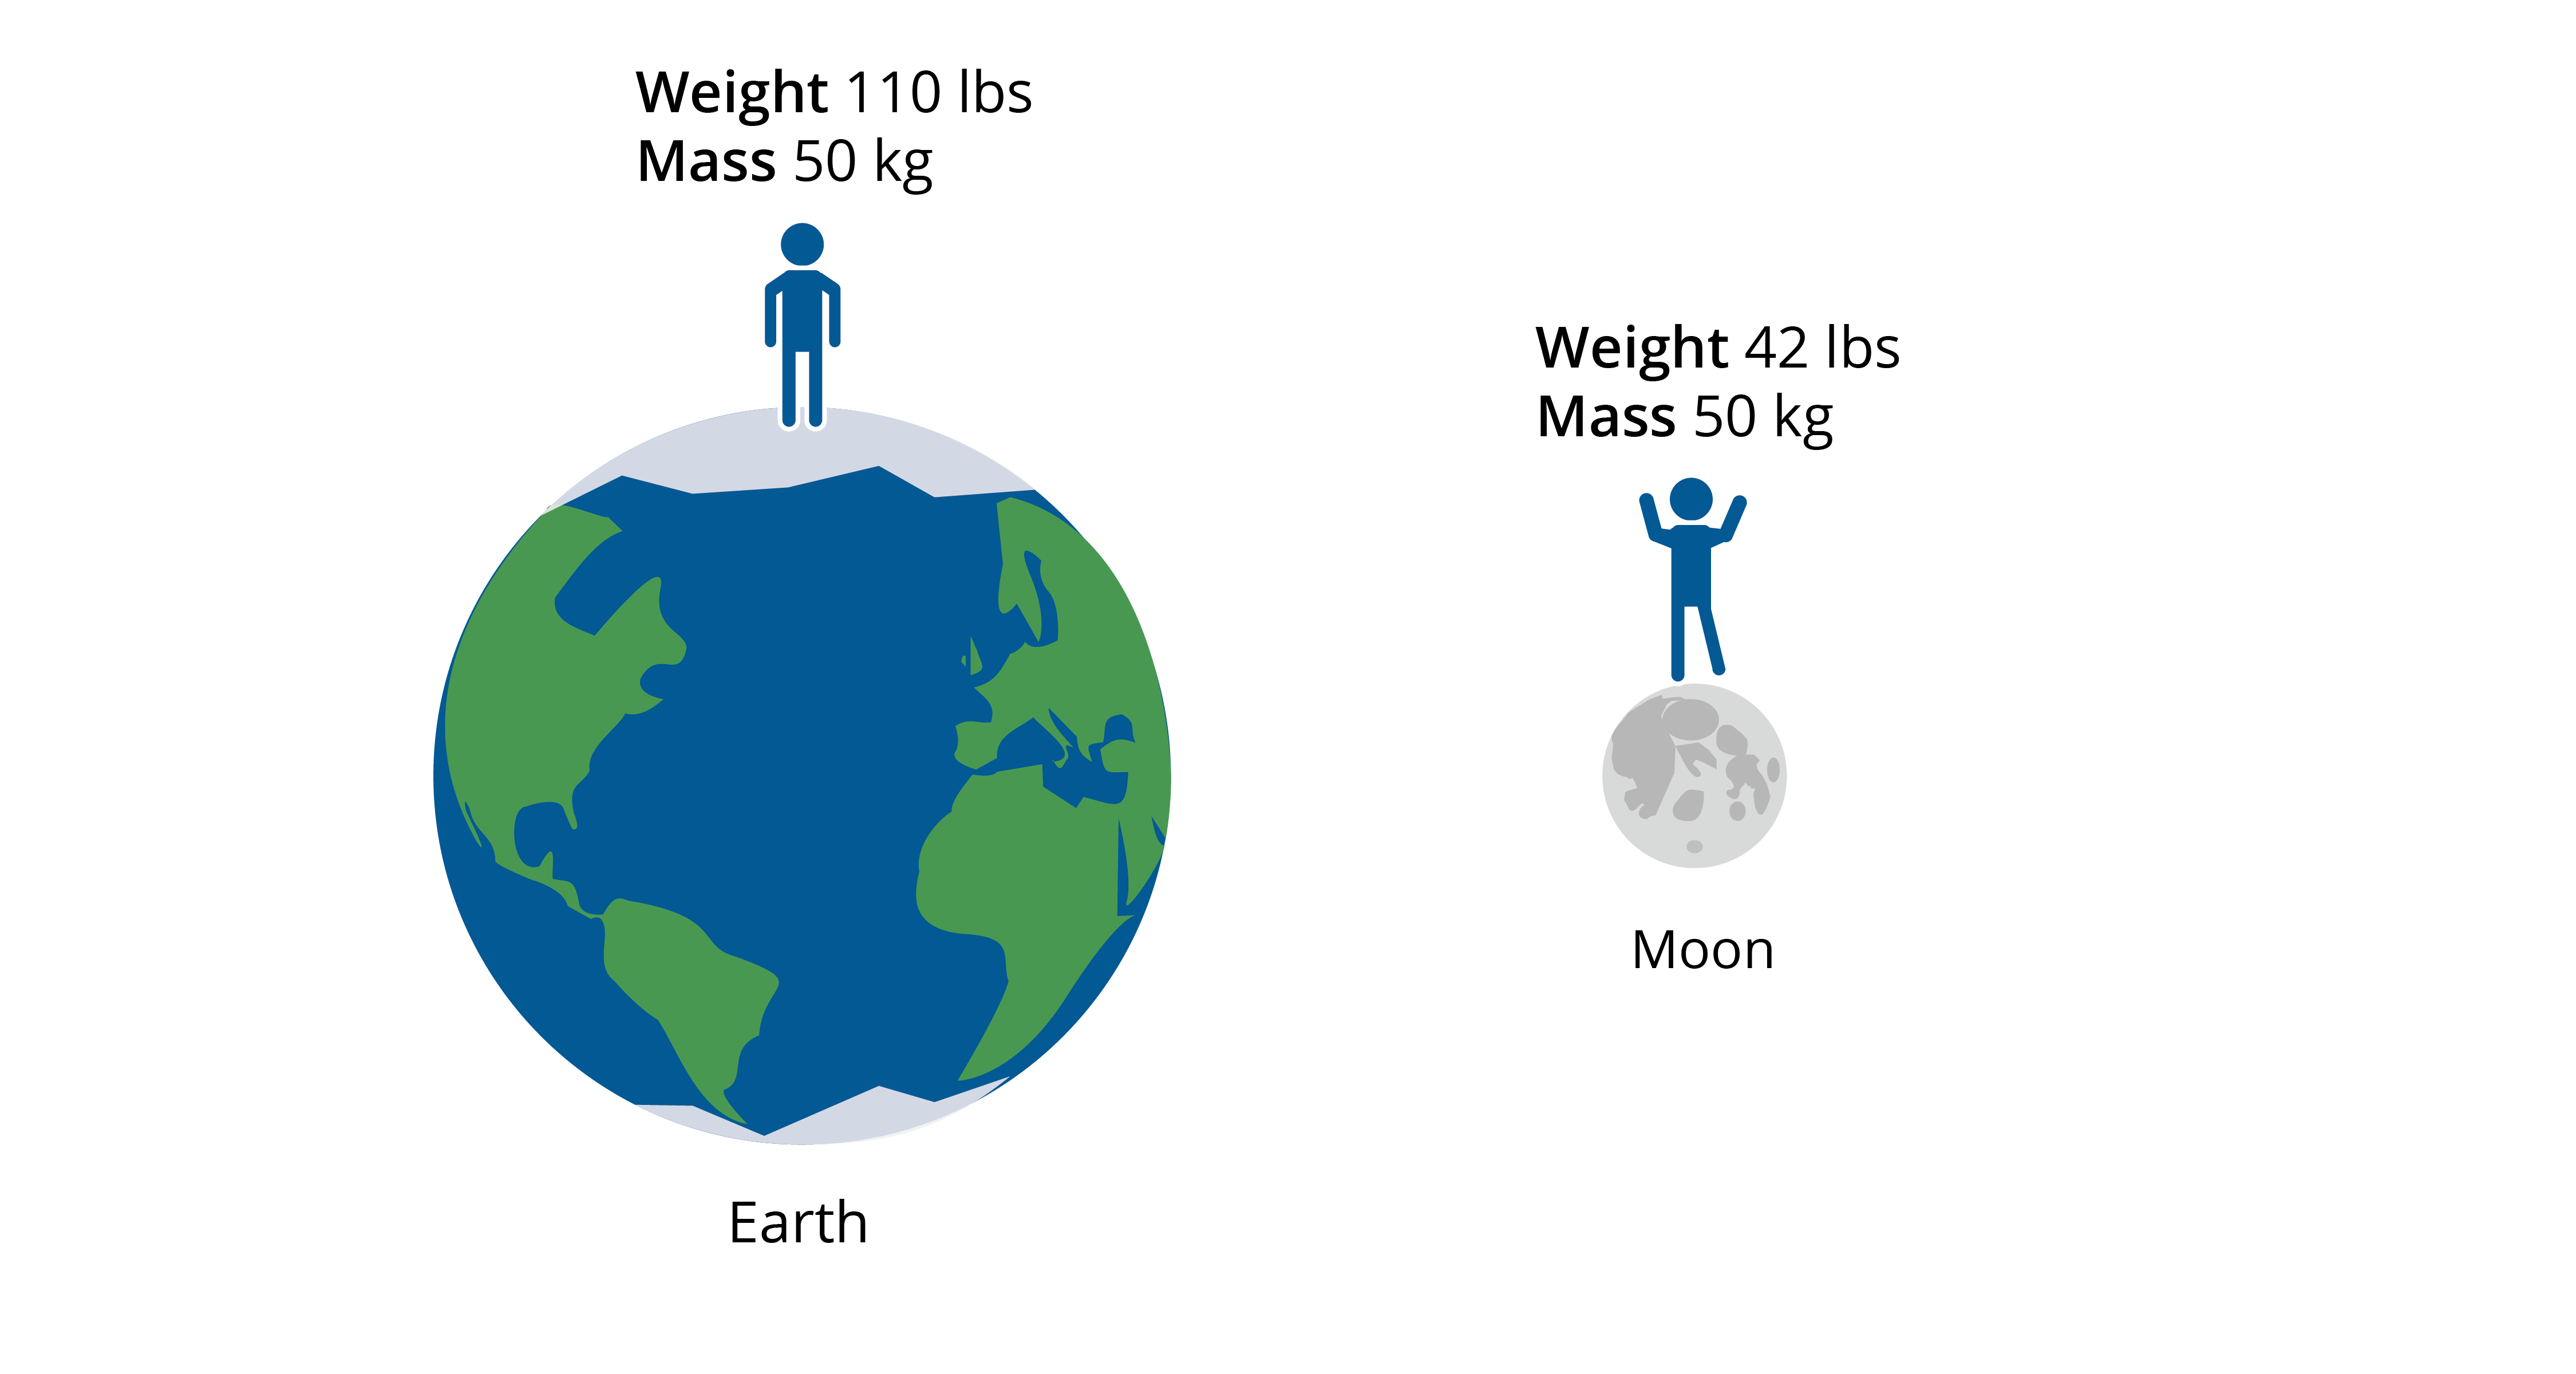
\includegraphics[width=0.6\textwidth]{massvweight.png}

But that potato has a mass of 0.45 kg anywhere in the universe.
